\section{Introduction}

\subsection{Background and Motivation}
Rapid global urbanization and the exponential growth of personal motor vehicles—particularly passenger cars and motorcycles—have led to severe urban traffic congestion in developing metropolises, such as Ho Chi Minh City, Vietnam. Constructing new physical road infrastructure requires substantial financial capital and extended timeframes, offering minimal immediate relief. Consequently, Intelligent Transportation Systems (ITS) powered by Artificial Intelligence (AI) have become an essential, cost-effective strategy for real-time traffic perception, adaptive signal control, and proactive congestion forecasting.

Figure~\ref{fig:traffic_jam} illustrates a representative urban traffic congestion scene in Ho Chi Minh City, highlighting extreme vehicle density and complex occlusions between passenger cars and motorcycles.

\begin{figure}[htbp]
\centering
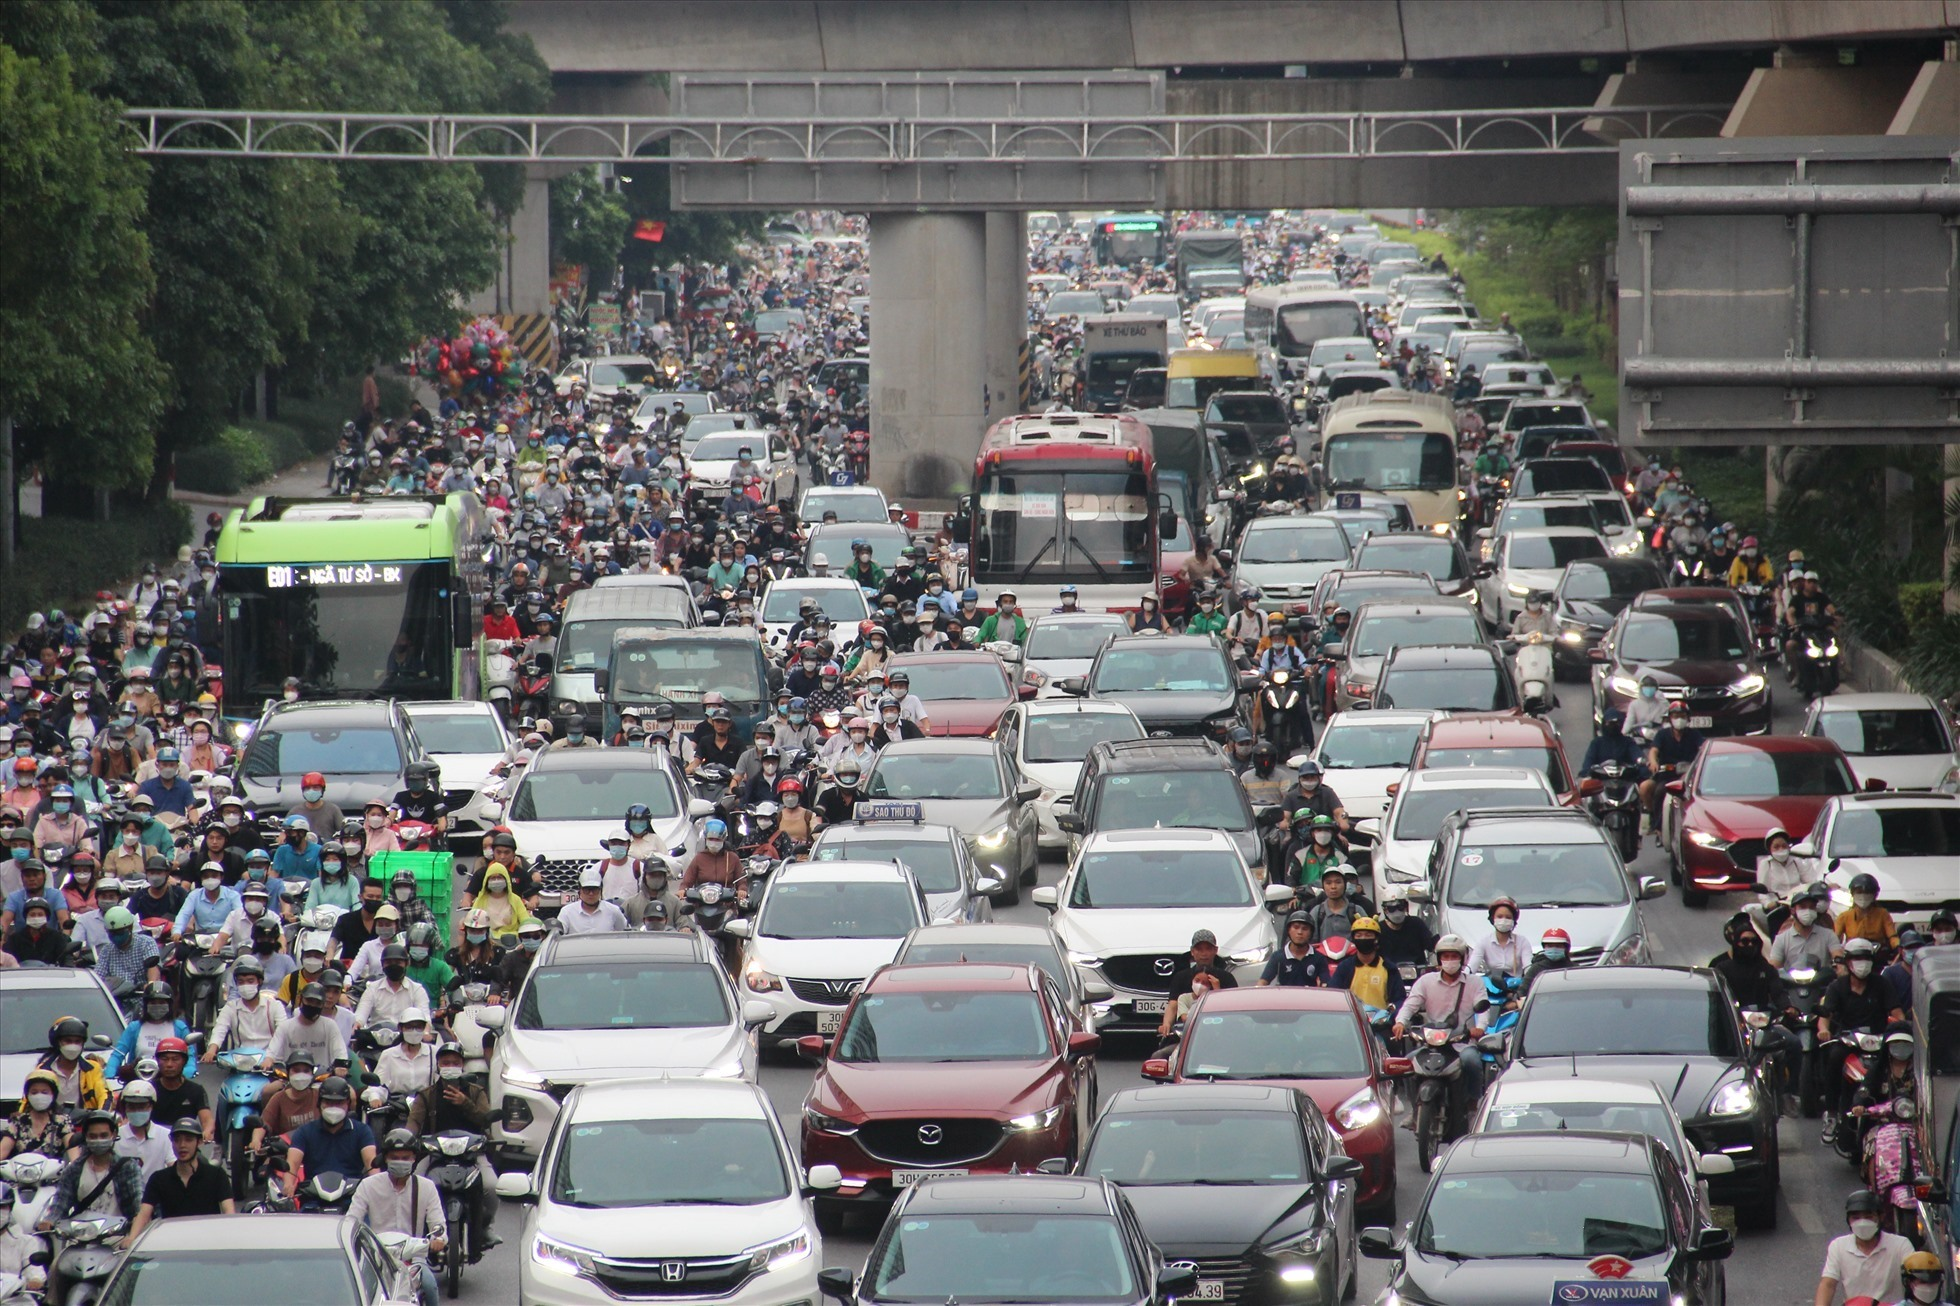
\includegraphics[width=\columnwidth]{fig/traffic_jam.jpg}
\caption{Urban traffic congestion in Ho Chi Minh City, Vietnam, illustrating extreme vehicle density and severe occlusions between passenger cars and motorcycles.}
\label{fig:traffic_jam}
\end{figure}

In modern urban environments, surveillance camera networks connected to public traffic portals offer high-coverage visual feeds at a fraction of the cost of physical induction loop sensors. However, transforming raw visual camera feeds into proactive city-wide traffic intelligence presents a complex multi-faceted challenge. To address this effectively, the overall urban traffic management framework is decomposed into two sequential sub-problems:
\begin{enumerate}
    \item \textbf{Sub-problem 1 (Camera-Level Perception):} Estimating real-time, category-specific vehicle counts (passenger cars and motorbikes) directly from individual camera feeds under complex outdoor conditions.
    \item \textbf{Sub-problem 2 (Network-Wide Forecasting):} Forecasting future traffic flow trends across the entire interconnected urban road network over multi-step time horizons ($t+1$ to $t+6$, corresponding to 5 to 30 minutes into the future).
\end{enumerate}

\subsection{Literature Review and Related Work}

\subsubsection{Visual Vehicle Estimation Methods (Sub-problem 1)}
Visual vehicle count estimation from surveillance cameras has evolved through three main computational paradigms:
\begin{itemize}
    \item \textbf{Object Detection (e.g., YOLO Series \cite{yolo}):} Detectors draw bounding boxes around individual vehicles per frame. Although effective in clear lighting and low-density traffic, object detection performance degrades severely under high traffic density, heavy vehicle occlusions, rain, fog, and nighttime lighting. Furthermore, per-vehicle bounding-box detection incurs high computational overhead.
    \item \textbf{Density Map Estimation (e.g., MCNN \cite{mcnn}, CSRNet \cite{csrnet}, CAN \cite{can}):} Fully Convolutional Networks (FCNs) map images to pixel-wise density maps, which are integrated to yield total vehicle counts. While resilient to crowd occlusions, density mapping cannot distinguish between different vehicle classes (e.g., separating motorbikes from cars) and requires labor-intensive pixel-level density annotations.
    \item \textbf{Direct Regression via Transfer Learning:} Direct regression maps camera images directly to continuous vehicle counts per class $[\hat{c}_{\text{car}}, \hat{c}_{\text{bike}}]^T$. By utilizing a modern \textbf{ConvNeXt-Tiny} backbone \cite{convnext} pre-trained on ImageNet-1K with a custom MLP regression head, direct regression retains category breakdown (like object detection) while maintaining high stability under dense occlusions (like density mapping).
\end{itemize}

\subsubsection{Time-Series Traffic Flow Forecasting Methods (Sub-problem 2)}
Early traffic forecasting relied on univariate statistical models (e.g., ARIMA \cite{arima}) or classical machine learning algorithms (e.g., Support Vector Regression SVR \cite{svr}). Modern deep learning approaches treat traffic forecasting through spatio-temporal deep neural networks \cite{dcrnn, wavenet, gman, agcrn, gnn_survey}:
\begin{itemize}
    \item \textbf{Sequential RNN Baselines (GCN-LSTM \cite{gcn, tgcn}):} Combine static Graph Convolutional Networks (GCN) \cite{gcn} with Recurrent Neural Networks (LSTM) or Gated Recurrent Units (GRU) \cite{tgcn}. However, sequential RNN backpropagation suffers from vanishing gradients, slow training, and an inability to parallelize across historical time windows.
    \item \textbf{Convolutional STGNNs (Standard STGCN \cite{stgcn}):} Yu et al. \cite{stgcn} introduced STGCN, combining Chebyshev Spectral Graph Convolutions (ChebNet) \cite{chebnet} with 1D Temporal Gated Convolutions (GLU). STGCN enables rapid parallel training; however, local 1D temporal convolutions have restricted receptive fields, making it difficult to capture dynamic, non-stationary long-term temporal dependencies.
\end{itemize}

\subsection{Problem Formulation and Inadequacy of Single-Node Forecasting}

A critical methodological insight of this study is that \textbf{single-node independent forecasting is fundamentally inadequate for urban traffic networks}.

If each camera location is treated as an isolated univariate time series and predicted independently (e.g., fitting a separate model per road segment), the forecasting system completely ignores spatial topological connectivity. Urban traffic flow is non-stationary and dynamic: congestion at one camera location rapidly spills over and propagates to connected downstream road segments via physical road connections and traffic bottlenecks \cite{ctm}. Predicting traffic at a single node without accounting for spatial graph topology leads to severe error propagation, particularly during peak hours or sudden traffic incidents.

Therefore, effective traffic forecasting requires modeling the entire camera network as a directed weighted spatial graph $\mathcal{G} = (\mathcal{V}, \mathcal{E}, W)$, where $\mathcal{V}$ represents the set of camera nodes ($N=608$ active camera stations across Ho Chi Minh City), $\mathcal{E}$ represents directed road connections, and $W$ is a Radial Basis Function (RBF) weighted distance matrix.

\subsection{Proposed TA-STGCN Framework vs. Baselines}
To address Sub-problem 2 and overcome the receptive field limitations of prior graph architectures \cite{stgcn, astgcn, stsgcn}, we propose \textbf{TA-STGCN} (Temporal Attention-Guided Spatio-Temporal Graph Convolutional Network). TA-STGCN integrates Chebyshev Spectral Graph Convolutions ($K=3$) \cite{chebnet}, 1D Temporal Gated Convolutions (GLU), and a \emph{Model-Level Multi-Head Temporal Self-Attention} module ($h=4$ heads) \cite{attention}. By applying multi-head temporal self-attention post-ST-Conv blocks, TA-STGCN functions as a dynamic low-pass filter that effectively down-weights high-frequency non-stationary temporal noise (such as sudden traffic signal shifts or transient visual camera glitches) while modeling multi-aspect temporal dependencies (immediate momentum, hourly periodicity, and daily patterns), resulting in superior convergence stability and smooth loss optimization across historical time windows ($T_{\text{in}} = 24$ steps = 120 minutes).

We evaluate TA-STGCN against two established baseline architectures:
\begin{enumerate}
    \item \textbf{Baseline 1 (GCN-LSTM):} Traditional sequential GNN combining 2 static GCN layers \cite{gcn} with a 2-layer LSTM ($364,198$ parameters - highest parameter capacity).
    \item \textbf{Baseline 2 (STGCN Baseline):} Standard 3-block STGCN \cite{stgcn} without attention mechanisms ($303,846$ parameters).
    \item \textbf{Proposed Model (TA-STGCN):} 2 ST-Conv blocks coupled with Model-Level Multi-Head Temporal Self-Attention \cite{attention} ($\mathbf{165,318 \text{ parameters}}$ - most lightweight architecture).
\end{enumerate}

\subsection{Main Contributions}
The main contributions of this paper are summarized as follows:
\begin{itemize}
    \item \textbf{Comprehensive End-to-End ITS Framework:} We design a unified two-stage ITS framework that seamlessly bridges camera-level visual perception (Sub-problem 1) with network-wide spatio-temporal graph forecasting (Sub-problem 2).
    \item \textbf{Annotated Camera Vehicle Image Dataset:} We contribute a real-world dataset of 6,000 manually annotated traffic camera images (4,000 Train, 1,000 Validation, 1,000 Test) collected across major intersections in Ho Chi Minh City, providing precise continuous count annotations for passenger cars and motorcycles under severe congestion.
    \item \textbf{Synchronized Urban Traffic Graph Dataset:} We construct a real-world 608-node spatio-temporal traffic graph dataset harvested via automated multi-threaded API pipelines from 657 CCTV cameras on the Ho Chi Minh City Traffic Portal, paired with topological road distances and RBF-weighted adjacency matrices.
    \item \textbf{TA-STGCN Architecture:} We design \emph{TA-STGCN}, introducing Model-Level Multi-Head Temporal Self-Attention \cite{attention} post-ST-Conv blocks to capture long-range temporal dependencies and smooth optimization trajectories without parameter inflation.
    \item \textbf{Rigorous 5-Seed Multi-Horizon Benchmark:} We conduct comprehensive multi-seed evaluations across 5 independent random seeds ($42, 100, 2024, 777, 999$) evaluating $H=6$ forecast horizons ($t+1$ to $t+6$). TA-STGCN achieves superior forecasting accuracy ($\text{MAE} = 3.1923 \pm 0.0112$, $\text{RMSE} = 4.3435 \pm 0.0142$) while being significantly more lightweight ($165,318$ parameters) than GCN-LSTM \cite{gcn} ($364,198$ parameters) and STGCN Baseline \cite{stgcn} ($303,846$ parameters).
\end{itemize}
